% !TeX root = ../main.tex
% !TEX spellcheck = en_GB

\chapter{Design}
\label{ch:Design}

\section{Overall}
\section{Sequence Diagrams}
The sequence diagrams (SD) below are meant to give an understanding of the inner workings of the \systemName.

Initiation of the system is described in \cref{fig:SD:init}.
It shows the µC initiating itself and then the external blocks.
The GPS module is polled until it returns valid location data. The time returned from the GPS allows the µC know the time and run the desired actions either at certain intervals, e.g. every 10 minutes, or at specific times, e.g. every full hour.
When valid data has been retrieved it is saved to the SD card and the GPS and GSM modules are put to sleep to conserve power.
The acquisition of GPS location is shown in \cref{fig:SD:getlocation}.
The GPS starts in a sleep mode and is awoken to find it's location.
When the location is found and is valid, the GPS is put back to sleep and the data is saved tot he SD card.
To upload data to the server, the GSM must be awoken and data must be retrieved from the SD card, as shown in \cref{fig:SD:upload}.
When the data has been sent the GSM is put back to sleep.

\begin{figure}
	\centering
	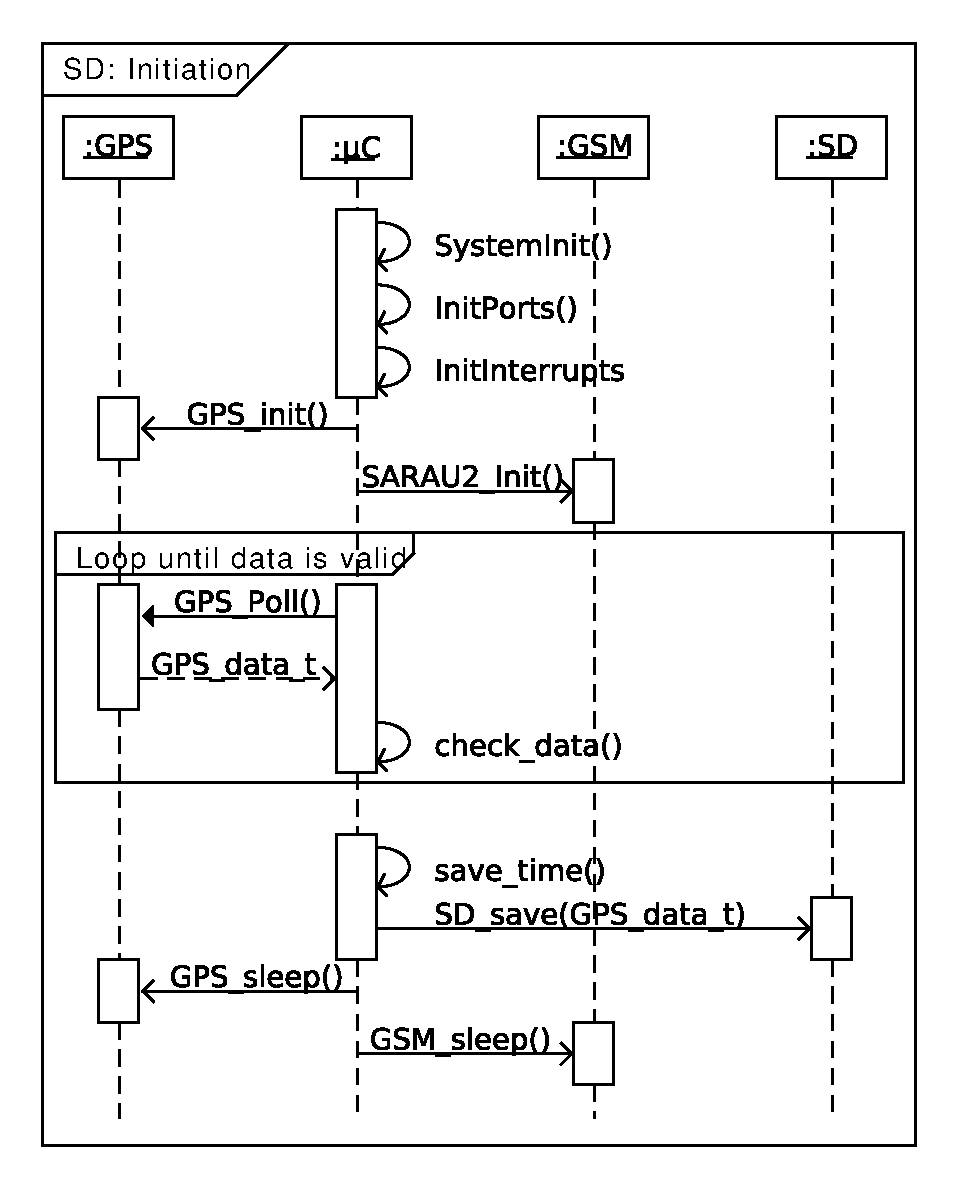
\includegraphics[width=0.7\linewidth]{gfx/Design/SD_init.pdf}
	\caption{Sequence diagram showing the initiation of the system.}
	\label{fig:SD:init}
\end{figure}

\begin{figure}
	\centering
	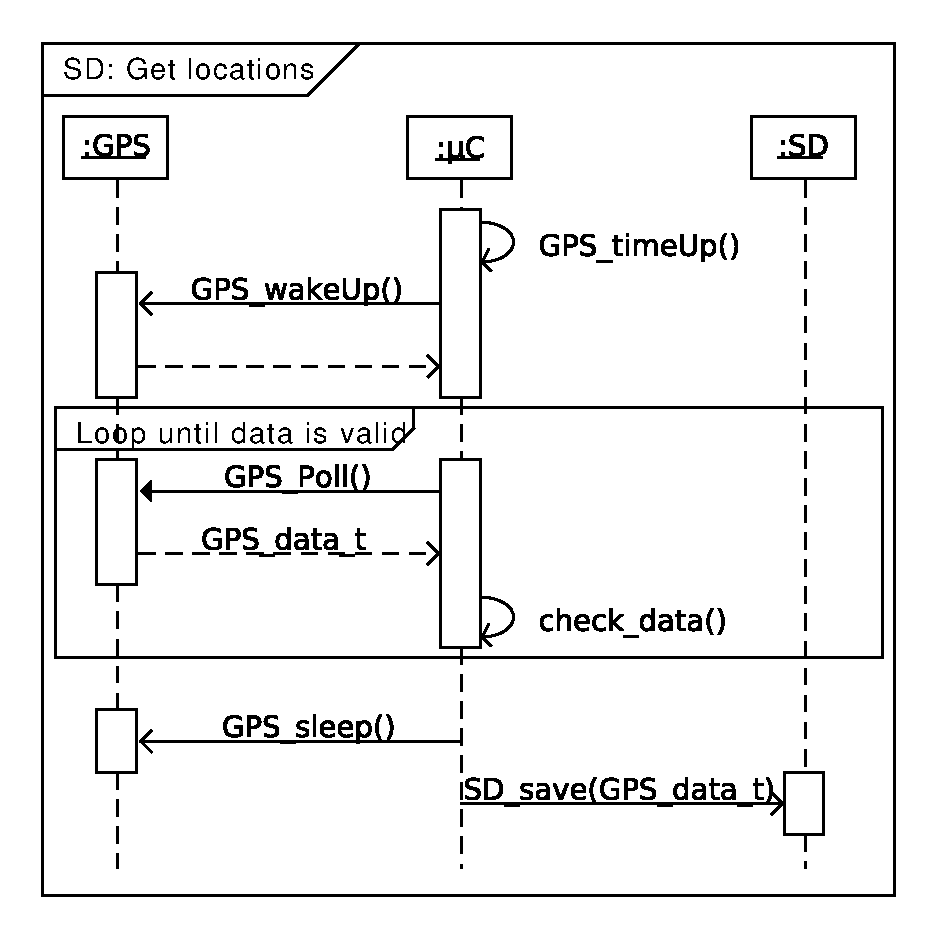
\includegraphics[width=0.7\linewidth]{gfx/Design/SD_getLocation.pdf}
	\caption{Sequence diagram describing the acquisition and saving of GPS data.}
	\label{fig:SD:getlocation}
\end{figure}

\begin{figure}
	\centering
	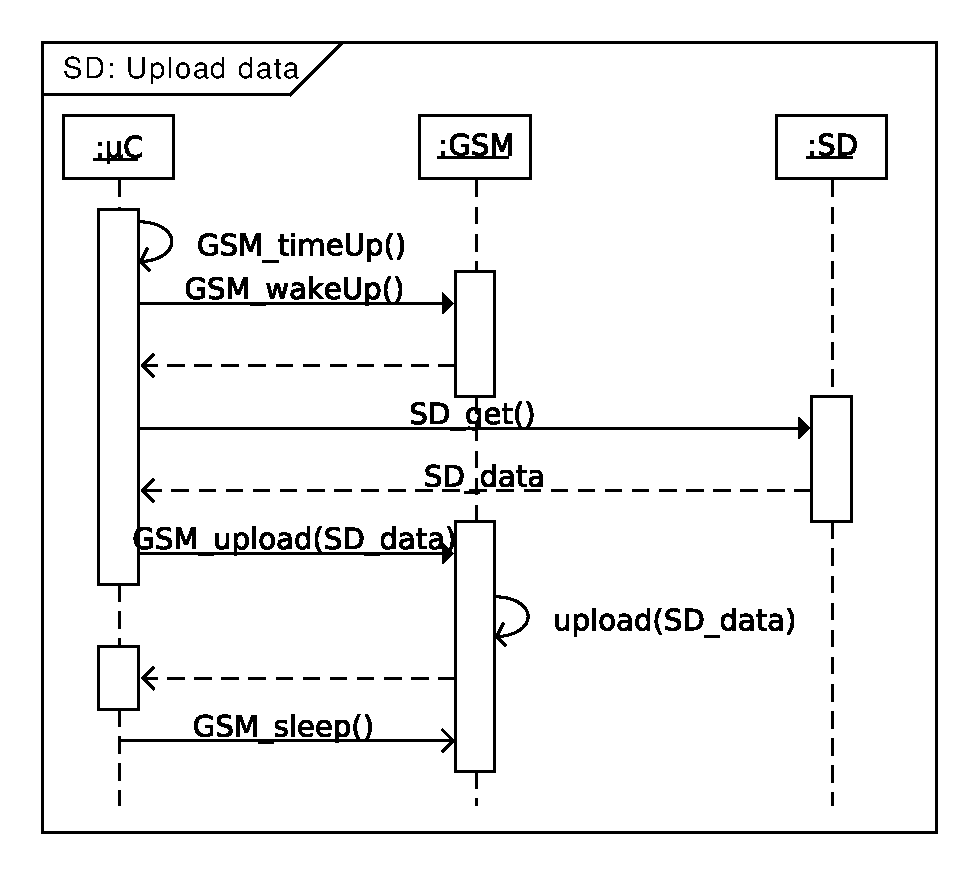
\includegraphics[width=0.7\linewidth]{gfx/Design/SD_Upload.pdf}
	\caption{Sequence diagram showing the process of sending saved data to the server.}
	\label{fig:SD:upload}
\end{figure}

\section{GSM - \SARA}

\subsection{UART}
Communication with the \SARA module, will be done through a UART connection. The module contains an ability to auto detect the baud rate of the first transmission, and use this baud rate to respond. In addition it supports the standard baud rates: \num{1200}, \num{2400}, \num{4800}, \num{9600}, \num{19200}, \num{38400} and 5 higher rates. \num{9600} baud was selected with focus on stability and the ability to debug the communications.

\subsection{AT Command Interface}
\fxnote{Describe - Sequence of AT commands}
From the analysis commands was found in order to set up the module, and send data through. The following section will run through the most important commands, what they do and how they are used. The commands are used in the order of table \fxnote{CHANGE TO sequence or float diagram with ref to \cref{app:sarau201}}

\section{GPS - \GPS}




\fxnote{Choices + Diagrammer}

\section{SD-card - \SDsock}


\section{UART - \SAMD}

\subsection{Clock}
\fxnote{Delvis Implementation}
The \SAMD is able to run with a clock frequency of \SI{48}{\mega\hertz}, but will during start up this is not active.
It is therefore necessary to activate not just the clock called \textit{DFLL48M} but also set up the reference clock, the generic clocks and the required multiplexers.

During operation \SAMD is able to maintain a given frequency through a DFLL(Digital Frequency Lock Loop).
This system relies on a secondary clock as a reference source for the main clock.
In the following list it is shown in what order the clocks and registers should be activated in order to get a stable system.

\begin{enumerate}
	\item Enable XOSC32K clock (External on-board 32.768Hz oscillator). Used as reference for \SI{48}{\mega\hertz} clock.
	\item Set Generic Clock Generator (1) source to XOSC32K.
	\item Active and set reference for Generic Clock Multiplexer.
	\item Enable DFLL48M.
	\item Set DFLL48M as source for Generic Clock Generator 0.
	\item Edit Pre scaler for OSCM clock to obtain \SI{8}{\mega\hertz}.
	\item Set OSC8M as source for Generic Clock Generator 3.
\end{enumerate} 

\subsection{BaudRate}
Both \SARA and \GPS supports the usage of auto baud rate detection, meaning that they will respond to a message in the same baud rate as they receive.
But due to consistency, both modules is set to the selected baud rate during their set up configuration. 
For simplicity a baud rate of \SI[per-mode = symbol]{9600}{\bit\per\second} was chosen, specification for the UART is shown in \vref{tab:BaudRate}.

\begin{table}[H]
	\begin{tabular}{ll}
		\hline 
		Baud Rate & 9600 \\ 
		\hline 
		Data Bits & 8 \\ 
		\hline 
		Parity & None \\ 
		\hline 
		Stop Bits & 1 \\ 
		\hline 
	\end{tabular}
	\centering
	\caption{Baud rate definition used for serial com ports on \SAMD.}
	\label{tab:BaudRate}
\end{table} 

\FloatBarrier